\documentclass[11pt,a4paper]{scrartcl}
\usepackage[left=1cm, right=1cm, bottom=1cm, top=1cm]{geometry}
\usepackage[dvipsnames]{xcolor}
\usepackage[T1]{fontenc}
\usepackage{fontspec}
\usepackage{graphicx, wrapfig, float, url}
\usepackage{xparse, fp, xifthen, expl3}
\usepackage{tikz}

\def\name{frosty}

\def\scale{0.24}

\def\num{109}

\def\vabstand{3ex}
\def\habstand{2ex}

% ########### get image dimensions #############
\newdimen\imagewidth
\newdimen\imageheight

\settowidth{\imagewidth}{%
	\includegraphics[scale=\scale]{\name}
}
\settoheight{\imageheight}{%
	\includegraphics[scale=\scale]{\name}
}	


\ExplSyntaxOn
% calculate amount of picture columns by dividing picture width by pagewidth
\NewDocumentCommand{\getlengthratio}{m m}
{
	\fp_eval:n { floor ( \dim_to_fp:n { #1 } / \dim_to_fp:n { #2 } , 0 ) }
}

% calculate amount of picture rows by dividing total number by cols
\NewDocumentCommand{\getrows}{m m}
{
	\fp_eval:n { floor ( { #1 } / { #2 } , 0 ) }
}

\NewDocumentCommand{\getpages}{m m}
{
	\fp_eval:n { ceil ( { #1 } / { #2 } , 0 ) }
}

\fp_new:N\test
\fp_set:Nn\test{1.2}
%\tl_new:N\test
%\tl_set:Nn\test{1.2}
\ExplSyntaxOff

% determine maximum amount of rows that fit on one page
\newcounter{maxrows}
\setcounter{maxrows}{\getlengthratio{\textheight}{\imageheight + \vabstand}}

% determine amount of columns
\newcounter{cols}
\setcounter{cols}{\getlengthratio{\textwidth}{\imagewidth + \habstand}}

% determine total amount of rows
\newcounter{rows}
\setcounter{rows}{\getrows{\num}{\thecols}}

% determine amount of full pages
\newcounter{pages}
\setcounter{pages}{\getrows{\therows}{\themaxrows}}

% determine amount of columns left
\FPeval\remcol{\num - \therows*\thecols}
\FPround\remcol{\remcol}{0}

% determine amount of rows left
\FPeval\remrow{\therows - \themaxrows*\thepages}
\FPround\remrow{\remrow}{0}


\begin{document}
%	debug
%	\Huge therows:\therows\\
%		themaxrows:\themaxrows\\
%		thepages:\thepages\\
%		thecols:\thecols\\
%		remrow:\remrow\\
%		remcol: \remcol\\
		
	\Huge\the\test
	\foreach \page in {1,...,\thepages}{
		\begin{figure}
		\centering
		\foreach \row in {1,...,\themaxrows}{
			\foreach \col in {1,...,\thecols}{
				\includegraphics[scale=\scale]{\name}\hspace{\habstand} 
			}
		\\[\vabstand]}
		\end{figure}
	\newpage }
	
	\ifthenelse{\equal{\remrow}{0}}{% do nothing
	}{
	\begin{figure}
		\centering
		\foreach \row in {1,...,\remrow}{
			\foreach \col in {1,...,\thecols}{
				\includegraphics[scale=\scale]{\name}\hspace{\habstand} 
			}
			\\[\vabstand]}
	\end{figure}
	}
	
	\ifthenelse{\equal{\remcol}{0}}{% do nothing
	}{
	\begin{figure}
	\centering
		\foreach \i in {1,...,\remcol}{
			\includegraphics[scale=\scale]{\name}\hspace{\habstand} }
	\end{figure}
	}


%		\foreach \i in {1,...,\remainder}{
%			\phantom{\includegraphics[scale=\scale]{\name}\hspace{\habstand}} }\\[\vabstand]

%		\foreach \col in {1,...,\col}{
%			\foreach \i in {1,...,\row}{
%				
\includegraphics[scale=\scale]{hungry}\hspace{\habstand} }\\[\vabstand]}
%		\foreach \col in {1,...,\col}{
%			\foreach \i in {1,...,\row}{
%				
\includegraphics[scale=\scale]{yeti}\hspace{\habstand} }\\[\vabstand]}
%		\foreach \col in {1,...,\col}{
%			\foreach \i in {1,...,\row}{
%				
\includegraphics[scale=\scale]{fire}\hspace{\habstand} }\\[\vabstand]}	
%		\foreach \col in {1,...,\col}{
%			\foreach \i in {1,...,\row}{
%				
\includegraphics[scale=0.3]{wizard}\hspace{\habstand} }\\[\vabstand]}	

%		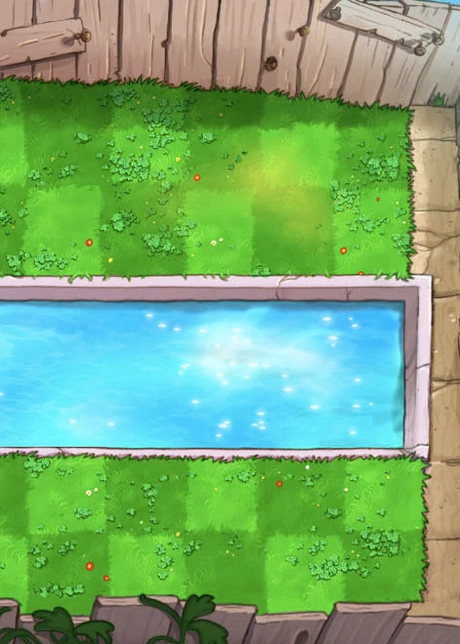
\includegraphics[scale=1.17]{pool_r}	
\end{document}